\documentclass[10pt, a4paper]{article}

\usepackage[paper=a4paper, left=2cm, right=2cm, bottom=2cm, top=2cm]{geometry}
\usepackage[utf8]{inputenc}
\usepackage[spanish]{babel}
\usepackage{graphicx}
\usepackage{multicol}
\usepackage[usenames,dvipsnames]{color}
\usepackage{amsmath}
\usepackage{verbatim}
\usepackage{footnote}
\usepackage{float}
\usepackage{amsfonts}
\usepackage{hyperref}
\usepackage{framed}
\usepackage{pdflscape}

\usepackage{pdfpages}

\usepackage{caratula}

\materia{Ingeniería de Software II}

\titulo{Trabajo Práctico 2}
\subtitulo{Developing \textsf{in-the-large} - Planificación}
\grupo{Grupo 5 - \emph{El nene está bien}}

\integrante{Martín Alejandro Miguel}{181/09}{m2.march@gmail.com}
\integrante{Iván Postolski}{216/09}{ivan.postolski@gmail.com}
\integrante{Juan Manuel Martinez Caamaño}{276/09}{jmartinezcaamao@gmail.com}
\integrante{Matías Incem}{396/09}{matias.incem@gmail.com}
\integrante{Pablo Gauna}{334/09}{gaunapablo@gmail.com}

\setcounter{tocdepth}{2}

\begin{document}

\maketitle
\tableofcontents
\newpage

\section{Introducción}

El presente informe constituye la planficación del proyecto \textbf{Twitteando para ahorrar} (TPA), que conforma una extensión del proyecto \textbf{Precio Justo} a partir de los intereses de parte de autoridades gubernamentales. Para este nuevo proyecto la metodología de trabajo utilizada se basará en la metodología \emph{RUP}, a causa del fuerte cambio en la escala de la aplicación respecto del trabajo anterior.  

\subsection{Caso de negocio}

El caso de negocio se modificó respecto del trabajo anterior principalmente en la escala del software a desarrollar. Esto incluye tanto un aumento en la base de usuarios de nuestra aplicación como en las funcionalidades a proveer. A continuación enunciamos el caso de negocio como una serie de objetivos a lograr:

\begin{itemize}
\item La información de precios no solo será obtenida de \emph{twitter}, sino que también de otras redes sociales (\emph{facebook}, \emph{pinterest}) y distintos sitios web (sitios de remate, sitios de supermercados, sitios de ofertas).
\item Los usuarios tendrán acceso a la aplicación mediante una interfaz web y una mobile. Las mismas deberán tener usabilidad accesible a toda la población, lo que implica que deben ser limpias y amigables.
\item La información recopilada también será provista de forma pública para otras aplicaciones, generando todo un nuevo lado de usabilidad a nuestra aplicación.
\item La presentación de información contará con más inteligencia, mostrando no solo productos que el usuario declaró como interesnates, sino también información de otros productos que se encuentren relacionados.
\item El uso de la aplicación será personalizable, dándole la oportunidad al usuario de definir niveles de confianza de las ofertas según su origen.
\item La detección de información falsa o sospechosa deberá ser muy robusta. Además, los detalles de la detección deberá ser visible.
\item Se continuará trabajando con una serie de \emph{productos} aceptados por la aplicación, pero estos se agruparán bajo el concepto de \emph{rubros}. La administración de productos y rubros tendrá como fin mejorar el manejo de información internamiente en el sistema.
\end{itemize}

\subsection{Detalles y restricciones}

Para el desarrollo de la aplicación deberemos tener en cuenta los siguientes detalles:

\begin{itemize}
\item No contaremos con servidores potentes para el procesamiento de datos, pero si con la cantidad que nos sea necesaria de equipos de escritorio.
\item Se nos exige que los datos se guarden en una base de datos \textbf{NOSQL}
\item Se nos exige que los servicios de provean desde \emph{la nube} utilizando servicios de \textbf{cloud computing}
\item Por limitaciones de presupuesto la aplicación debe ser capaz de generar ingresos en el corto plazo
\item Se nos sugiere el servicio SpamBust para lograr la detección de ofertas falsas. No obstante el servicio es pago y deberá ser reemplazado en la brevedad.
\item Las funcionalidades de preferencias y reputación de usuarios deberán ser visibles para los \emph{stakeholders} en un plazo de dos meses.
\end{itemize}

\subsection{Diccionario de términos}

\begin{itemize}
\itemsep1pt\parskip0pt\parsep0pt
\item
  \textbf{Oferta}: Información sobre donde comprar un producto X y a qué
  precio.
\item
  \textbf{Usuario autenticado}: Usuario del cual el sistema tiene
  seguridad quién es.
\end{itemize}


\section{Análisis inicial de proyecto}

\subsection{Casos de uso}

En esta etapa del proyecto están definidos los siguientes \emph{casos de uso} como descripción completa de la aplicación desde el punto de vista de las funcionalidades que tendrá.

\subsubsection{CU1: Obteniendo informacion de internet}

\textbf{Descripción}: El sistema colecta la información de los distintos
medios, la procesa, y la almacena para luego ser provista a los
usuarios.

\subsubsection{CU2: Se consulta información a travéz de el API publica.}

\textbf{Descripción}: Clientes externos pueden consultar a nuestro
sistema por precios que recopilamos de distintos medios a través de un
servicio público (API) ofrecido por nuestro sistema.

\subsubsection{CU3: El usuario consulta precios a través de una interfaz
amigable}

\textbf{Descripción}: El usuario accede a una aplicación de celular
propia de \emph{twitteando para ahorrar} a través de la cual puede
consultar por precios para distintos productos.

\subsubsection{CU4: Se realizó una consulta por un producto, y el
dispositivo sin tener conexión, logra responder la consulta de alguna
forma medianamente satisfactoria.}

\textbf{Descripción}: El usuario accede a la aplicación de celular
\emph{twitteando para ahorrar} sin tener conectividad a internet y
recibe precios de los productos deseados y los relacionados a estos. La
información provista al usuario podría estar limitada respecto de lo que
vería si tuviera conectividad, pero esto no debería ser notado por el
mismo.

\subsubsection{CU5: ABM de rubros habilitados.}

\textbf{Descripción}: Ciertos usuarios particulares del sistema pueden
acceder al mismo para agregar nuevos rubros o modificar o borrar
existentes.

\subsubsection{CU6: ABM de productos en un rubro.}

\textbf{Descripción}: Ciertos usuarios particulares del sistema pueden
acceder al mismo para agregar nuevos productosi o modificar o borrar
existentes. También pueden redefinir la pertenencia de un producto a uno
o más rubros.

\subsubsection{CU7: Si realizo una consulta por un producto A, obtengo
ofertas de este producto.}

\textbf{Descripción}: El usuario consulta por un producto A dentro de
los habilitados en algún rubro y recibe información de donde comprarlo y
a qué precio.

\subsubsection{CU8: Si realizo una consulta por un producto A y este no
está se le informa al usuario.}

\textbf{Descripción}: El usuario consulta por un producto A que no está
habilitado en ningún rubro y es informado que el sistema no posee
información sobre donde comprar el mismo.

\subsubsection{CU9: Si realizo una consulta por un producto A, y se
considera que puede sustituirse por B, tambien se muestran ofertas de
B.}

\textbf{Descripción}: El usuario consulta por un producto A dentro de
los habilitados en algún rubro y se definió que puede sustituirse por el
producto B, luego el usuario recibe información de donde comprar A y
donde comprar B y a qué precio.

\subsubsection{CU10: Si realizo una consulta por un producto A, que se
considera asociado con B, tambien se muestran ofertas de B.}

\textbf{Descripción}: El usuario consulta por un producto A dentro de
los habilitados en algún rubro y se definió que está asociado con el
producto B, luego el usuario recibe información de donde comprar A y
donde comprar B y a qué precio.

\subsubsection{CU11: Si realizo una consulta por un producto A y soy un
usuario autentificado, las ofertas recibidas se priorizan acorde a mis
preferencias de confianza.}

\textbf{Descripción}: Dentro de las ofertas relacionadas al producto A
que conoce el sistema, se mostrarán primero aquellas cuya fuente yo haya
declarado de mayor confianza, luego las de fuentes con menor confianza y
no se mostrará ninguna oferta cuya fuente declaré como no confiable.

\subsubsection{CU12: Mostrando publicidades}

\textbf{Descripción}: Cuando el usuario utiliza la aplicación movil
visualiza, aparte de los resultados de su consulta, propaganda de los
spónsores de \emph{twitteando para ahorrar}.

\subsubsection{CU13: Detectando ofertas falsas}

\textbf{Descripción}: Al recopilar datos de precios en internet, el
sistema es capaz de detectar si la información es sospechosa y marcarla
como tal, para futura revisión. Además el sistema recopila todas las
evidencias encontradas para sospechar de los datos.

\subsubsection{CU14: Siendo martes se publica un informe de ofertas
falsas}

\textbf{Descripción}: Cada martes el sistema arma y publica un informe
con los productos sobre los cuales se encontraron precios dudosos junto
con la evidencia que genera la sospecha. Este informe debe estar
disponible para revisión por usuarios externos selectos.

\subsubsection{CU15: Se prepara un informe con las estadisticas de
ofertas detectadas como falsas.}

\textbf{Descripción}: Al mismo tiempo que el usuario comienza a ingresar
una consulta en la aplicación movil, la aplicación se anticipa a los
deseos del usuario para mostrarle rápidamente precios de productos que
podríán responder a la consulta que se está formulando.

\subsubsection{CU16: El usuario se autentica con el sistema}

\textbf{Descripción}: El usuario de la aplicación movil puede utilizar
alguna cuenta de un servicio asociado con OpenID (google, yahoo,
facebook y otro) para autenticarse en la aplicación. A partir de ese
momento la aplicación sabe quién es el usuario y puede utilizar la
información que tiene del mismo para proveerle funcionalidades más
avanzadas.

\subsubsection{CU17: Un usuario autentificado puede votar por la validez
de una oferta.}

\textbf{Descripción}: Un usuario ya autenticado en el sistema elije una
oferta y la marca como válida o inválida. Esto afecta la reputación del
usuario o fuente que dio origen a la oferta para facilitar la detección
de ofertas sospechosas.


\subsection{Análisis de riesgos}

A su vez se realizó un análisis de los posibles problemas que pueden surgir en el desarrollo del sistema. A continuación presentamos la listas de riegos analizados.

\subsubsection{Riesgo1:}

\begin{itemize}
\itemsep1pt\parskip0pt\parsep0pt
\item
  \textbf{Descripción}: Por falta de definiciones claras y consisas el
  código desarrollado no cumple con las expectativas de los stakeholders
  y se vuelve necesario modificarlo. Se consideran particularmente
  riesgosas las definiciones en: criterios de sustitución y asociación,
  información a recuperar, prioridad de los usuarios por la información.
\item
  \textbf{Probabilidad}: Alta
\item
  \textbf{Impacto}: Alto
\item
  \textbf{Exposición}: Alta
\item
  \textbf{Mitigación}: Acordar fechas límites para la presentación de
  documentación definiendo mejor cada caso en particular. Se aislarán y
  se implementarán los modulos correspondientes a estas caracteristicas
  de forma que su modificación resulte lo mas rapida posible.
  (Modificabilidad)
\item
  \textbf{Plan de contingencia}: Se estiran los períodos del proyecto
  para poder realizar las modificaciones necesarias.
\end{itemize}

\subsubsection{Riesgo2:}

\begin{itemize}
\itemsep1pt\parskip0pt\parsep0pt
\item
  \textbf{Descripción}: Falta de dinero para financiar el proyecto.
\item
  \textbf{Probabilidad}: Media
\item
  \textbf{Impacto}: Alto
\item
  \textbf{Exposición}: Alta
\item
  \textbf{Mitigación}: Conseguir sponsor, lo antes posibles, para que el
  proyecto sea auto-sostenible.
\item
  \textbf{Plan de contingencia}: Resignar funcionalidades del proyecto
  que requiera mucha inversión para reducir los costos.
\end{itemize}

\subsubsection{Riesgo3:}

\begin{itemize}
\itemsep1pt\parskip0pt\parsep0pt
\item
  \textbf{Descripción}: El hardware disponible no es suficiente para
  soportar TODAS las funcionalidades a cumplir (extraer datos,
  publicarlos mediante la api, predecir los deseos del usuario,
  verificar los datos recibidos, generar información de auditoría).
\item
  \textbf{Probabilidad}: Media
\item
  \textbf{Impacto}: Alto
\item
  \textbf{Exposición}: Alta
\item
  \textbf{Mitigación}: Aprender a utilizar correctamente los recursos a
  nuestro alcance, en este caso los equipos de escritorio. Entrenar a
  los desarrolladores en técnicas de cómputo paralelo.
\item
  \textbf{Plan de contingencia}: Resignar alguna de las funcionalidades.
\end{itemize}

\subsubsection{Riesgo4:}

\begin{itemize}
\itemsep1pt\parskip0pt\parsep0pt
\item
  \textbf{Descripción}: Inconvenientes con el servicio de spambust que
  nos deja sin esta funcionalidad. (E.g.: sube el precio, problemas de
  servicio por su parte).
\item
  \textbf{Probabilidad}: Baja
\item
  \textbf{Impacto}: Alto
\item
  \textbf{Exposición}: Media
\item
  \textbf{Mitigación}: Implementar, lo antes posible, un servicio propio
  que remplace el de spambust.
\item
  \textbf{Plan de contingencia}: Dejar de detectar el spam o detectarlo
  en menor medida con una implementación fácil y rápida pero no tan
  efectiva.
\end{itemize}

\subsubsection{Riesgo5:}

\begin{itemize}
\itemsep1pt\parskip0pt\parsep0pt
\item
  \textbf{Descripción}: Un miembro abandona el equipo de trabajo.
\item
  \textbf{Probabilidad}: Media
\item
  \textbf{Impacto}: Medio
\item
  \textbf{Exposición}: Media
\item
  \textbf{Mitigación}: Particionado al sistema en `modulos' simples con
  una única responsabilidad y alta cohesión interna, y manteniendo la
  documentación de la arquitectura del sistema actualizada, de forma que
  al incorporar un remplazo, la curva de aprendizaje del sistema se vea
  reducida.
\item
  \textbf{Plan de contingencia}: Contratar remplazo.
\end{itemize}

\subsubsection{Riesgo6:}

\begin{itemize}
\itemsep1pt\parskip0pt\parsep0pt
\item
  \textbf{Descripción}: Los deseos del usuario sobre la aplicación no
  son los esperados por los stakeholders y es necesario cambiar
  drásticamente la funcionalidad.
\item
  \textbf{Probabilidad}: Media
\item
  \textbf{Impacto}: Media
\item
  \textbf{Exposición}: Media
\item
  \textbf{Mitigación}: Tener una versión beta de la aplicación de
  usuario para tener feedback lo antes posible y poder agregar las
  modificaciones de forma suave y sin desperdiciar tiempo de trabajo.
\item
  \textbf{Plan de contingencia}: Hacer estudios de marketing para
  comprender realmente las necesidades del usuario.
\end{itemize}

\subsubsection{Riesgo7:}

\begin{itemize}
\itemsep1pt\parskip0pt\parsep0pt
\item
  \textbf{Descripción}: Desconocimiento de las tecnologías a usar:
  OpenID, base de datos nosql, webmining, sms, cloud computing, etc. que
  podría llegar a ocasionar retrasos inesperados en el proyecto.
\item
  \textbf{Probabilidad}: Media
\item
  \textbf{Impacto}: Bajo
\item
  \textbf{Exposición}: Baja
\item
  \textbf{Mitigación}: Dedicar horas de aprendizaje, lo antes posible,
  para cada tecnología y saber de antemano los problemas que podrían
  suceder.
\item
  \textbf{Plan de contingencia}: Contratar gente especializada en las
  tecnologías.
\end{itemize}

\subsubsection{Riesgo8:}

\begin{itemize}
\itemsep1pt\parskip0pt\parsep0pt
\item
  \textbf{Descripción}: Debido a los tiempos acotados requerido para
  sacar al mercado el producto, los módulos podrían carecer del testing
  adecuado.
\item
  \textbf{Probabilidad}: Media
\item
  \textbf{impacto}: Bajo
\item
  \textbf{Exposición}: Baja
\item
  \textbf{Mitigación}: Mantener un mínimo nivel de testing requerido en
  cada módulo.
\item
  \textbf{Plan de contingencia}: Reparar bugs y mejorar los test del
  módulo.
\end{itemize}


\subsection{Intereses y prioridades}

En vista de los análisis presentados resumimos una serie de intereses principales y criterios de priorización de tareas que serán usados para la planificación del proyecto. 

En primer lugar consideramos que debe haber una versión de la nueva aplicación movil funcionando lo antes posible, aunque no poseea la funcionalidad completa. Esto está motivado por la mitigación de dos riegos importantes que son la incompatibiliad de la aplicación movil con los usuarios de la misma y la falta de dinero para el proyecto. Con una versión de la aplicación funcionando, es más fácil evaluar las preferencias de los usuarios y encontrar dificultades en su uso. Luego, dado que todavía estamos en las primeras etapas de desarrollo será mucho más facil corregir los requerimientos. La idea es mantener una fuerte atención sobre la recepción de la aplicación por parte de los usuarios, para lograr atender el interés de uso masivo.

A su vez, en una aplicación andando podemos mostrar publicidades de distintos sponsores, empezando a conseguir financiación y mitigando el importante riesgo de falta de dinero, que podría cancelar el proyecto completamente.

Por otra parte, dada la importancia de la funcionalidad de detección de ofertas sospechosas, será importante integrar \textbf{SpamBust} al sistema lo antes posible, por lo que priorizará capacitar al personal en su uso. A su vez, se deberán priorizar las tareas de análisis y desarrollo del sistema que reemplazará a \textbf{SpamBust}, dado el riesgo que implica depender de un servicio externo, así como los gastos que acarrea. 

Debidas las limitaciones de hardware que tenemos consideramos clave hacer buen uso de nuestros recursos, ya que de otra forma el sistema podría tener problemas para proveer la performance deseada frente a la escala de la base de usuarios que tendrá. Para lograr esto, se entrenará al equipo de trabajo en metodologias y teconologías de \emph{computación distribuída}, que permitirán aprovechar los equipos de escritorio con los que contamos. 

Finalmente, los principales \emph{stakeholders} del proyecto hicieron enfasís en que quieren ver la funcionalidad de reputación y preferencias de usuario funcionando lo antes posible. Estas funcionalidades están representadas en los \emph{casos de uso} 11 y 17. Las tareas relacionadas con los mismos serán priorizadas.

\section{Plan de proyecto}

\subsection{Plan de iteraciones}

Con el análisis realizado y las prioridades definidas se distribuyeron las funcionalidades de la aplicación en distintas iteraciones, acorde a la metodología \emph{RUP}. En las primeras iteraciones se encuentran aquellos \emph{casos de uso} que nos permiten mejor mitigar riesgos. En estas el análisis fue más detallado y se definieron tareas administrativas y operativas que serán necesarias. La visibilidad de las siguientes iteraciones es más reducida y deberá mejorar avanzado el proyect. 

Para el final de la fase de elaboración se espera tener una versión de la aplicación movil funcionando y aclaradas las definiciones de temas críticos como las preferencias de confianza y el sistema de reputación. La etapa de elaboración consiste de dos iteraciones de 6 semanas cada una.

Para la fase de construcción la planificación de iteraciones fue más aproximada y deberá ser corregida en el plan de desarrollo actualizado que tendremos al finalizar la fase de elaboración. Se calcularon 3 iteraciones de construcción considerando 5 programadores que trabajan 5 horas por día 20 días en un mes.

En el plan presentado a continuación se separaron en iteraciones las distintas funcionalidades a implementar, representadas por los \emph{casos de uso}. El detalle de qué tareas y qué subcomponentes serán necesarios para lograr el sistema completo fue analizado mediante la técnica de \textbf{Work Breakdown Structure}.  El esquema correspondiente puede verse en la sección siguiente.

\begin{enumerate}
	\item $\bullet$ $\rightarrow$ \textit{Caso de uso}.
	\item $\circ$ $\rightarrow$ \textit{Tarea}.
\end{enumerate}

\begin{center}
	\begin{tabular}{| c | p{10cm} | c |}
		\hline
		\textbf{Primera iteración}& $\circ$ Obteniendo información definida de Twitter. &  \\
								  & $\bullet$ Almacenando datos obtenidos de distintos sitios de internet. & \\
								  & $\bullet$ Si realizo una consulta por un producto A, obtengo ofertas de este producto. & \\
								  & $\bullet$ Mostrando publicidades en la aplicación. & \\
								  & $\circ$ Establecer una primera interfaz de fácil implementación. & \\
								  & $\circ$ Diseño conceptual del sistema. & \\ 
								  & $\circ$ Realización de WBS. & \\
								  & $\circ$ Primera revisión del caso de negocio, objetivos y requerimientos. & \\
								  & $\circ$ Análisis de riesgos. & \\
								  & $\circ$ Definición y priorización de casos de uso, documentando los tiempos esperados para los casos de uso más prioritarios. & \\
								  & $\circ$ Definir junto a los stakholder los atributos de calidad del sistema. & \\
								  & $\circ$ Diseño de la Arquitectura, teniendo en cuenta las restricciones a las tecnologías impuestas por los stakholder. & \\

		\hline
		\textbf{Segunda iteración}& $\bullet$ El usuario se autentifica con el sistema. &  \\
								  & $\bullet$ Un usuario autentificado puede votar la validez de una oferta. &  \\
								  & $\bullet$ Si realizo una consulta por un producto A y soy un usuario autentificado, las ofertas recibidas se priorizan acorde a mis preferencias de confianza. & \\
								  & $\bullet$ ABM de rubros habilitados. & \\
								  & $\bullet$ ABM de productos en un rubro. & \\
								  & $\bullet$ Si realizo una consulta por un producto A y este no esta, se le informa al usuario. & \\

		\hline
		\textbf{Tercera iteración}& $\bullet$ Se realizó una consulta por un producto, y el dispositivo sin tener conexión, logra responder la consulta de alguna forma medianamente satisfactoria. & \\
								  & $\bullet$ Detectando ofertas falsas. & \\
								  & $\bullet$ Siendo martes se publica un informe de ofertas falsas. & \\
								  & $\bullet$ Se prepara un informe con las estadisticas de ofertas detectadas como falsas. & \\

		\hline
		\textbf{Cuarta iteración}& $\bullet$ El usuario consulta precios a través de una interfaz amigable en su celular. & \\
								 & $\bullet$ Si realizo una consulta por un producto A, y se considera que puede sustituirse por B, tambien se muestran ofertas de B. & \\
								 & $\bullet$ Si realizo una consulta por un producto A, y se considera que puede sustituirse por B, tambien se muestran ofertas de B. & \\
								 & $\bullet$ Si realizo una consulta por un producto A, que se considera asociado con B, tambien se muestran ofertas de B. & \\

		\hline
		\textbf{Quinta iteración}& $\bullet$ Almacenando datos obtenidos de distintos sitios de internet. & \\
								 & $\bullet$ El usuario consulta precios a través de una interfaz amigable en su computadora. & \\
								 & $\bullet$ Se consulta información a travéz de el API publica. & \\

		\hline
	\end{tabular}
\end{center}


\subsection{Work Breakdown Structure}



\newcommand{\escaladefault}{0.85}

Incluimos un WBS híbrido de procesos y productos, para ilustrar los subcomponentes del proyecto. 

En la primera capa de este WBS, se divide al sistema principal en subsistemas menores, cada uno de estos encargado
de una tarea en particular.

En el WBS, se describen los procesos necesarios para poder desarrollar con exito estos subsistemas. Ademas 
de los subsistemas, algunos subproductos como documentaciones y modulos auxiliares necesarios para el desarrollo 
de un sistema respectivo son declarados.

Es esperable que los procesos declarados dentro de este diagrama, conforme avance el proyecto, sean sintetizados en tareas 
a realizar en alguna iteracion en particular.

El WBS define dependencias tentativas en el proyecto, sin embargo, estas estan sujetas a cambios y es esperable que deban 
ajustarse a lo largo del proyecto.

Vale destacar que para el desarrollo de ciertos productos, de los cuales esperamos que esten sujetos a cambios, se tuvo en 
cuenta un proceso de "correcion de requerimientos".

\begin{figure}[H]
\centering
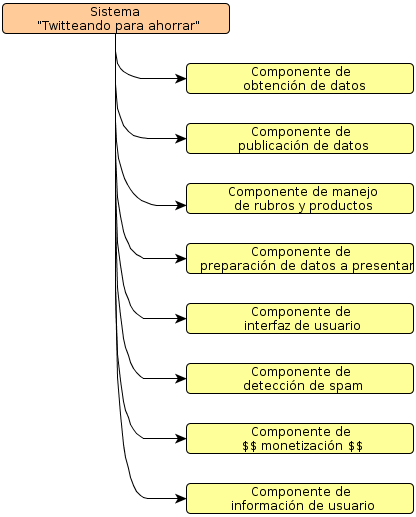
\includegraphics[scale=\escaladefault]{graficos/wbs/primera_capa.png}
\caption{Vista general del WBS: componentes del proyecto}
\end{figure}

\begin{figure}[H]
\centering
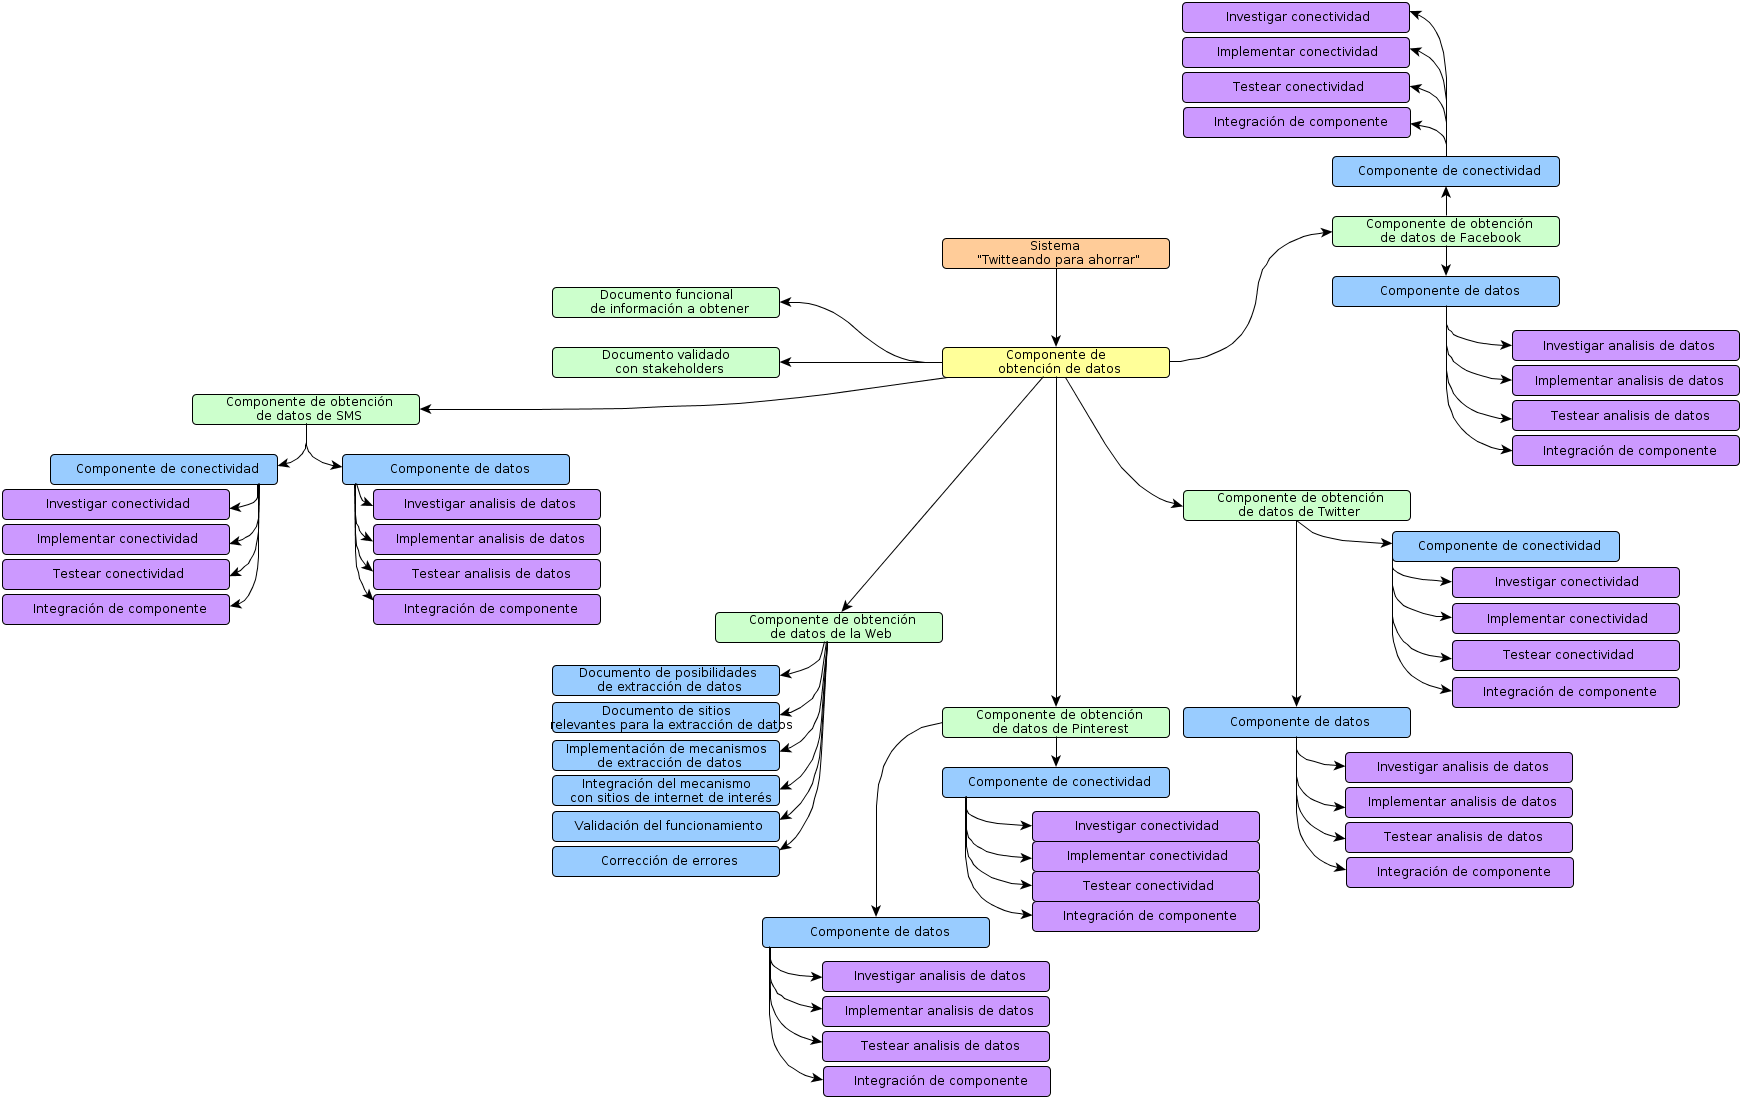
\includegraphics[scale=\escaladefault]{graficos/wbs/comp_obtencion_datos.png}
\caption{Componente de obtención de datos}
\end{figure}

\begin{figure}[H]
\centering
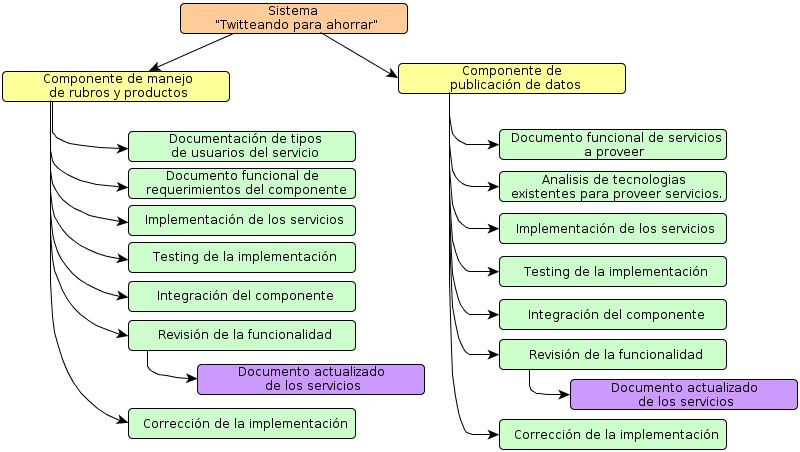
\includegraphics[scale=\escaladefault]{graficos/wbs/comp_rubros_y_api.png}
\caption{Componente de publicación de datos y componente de rubros y productos}
\end{figure}

\begin{figure}[H]
\centering
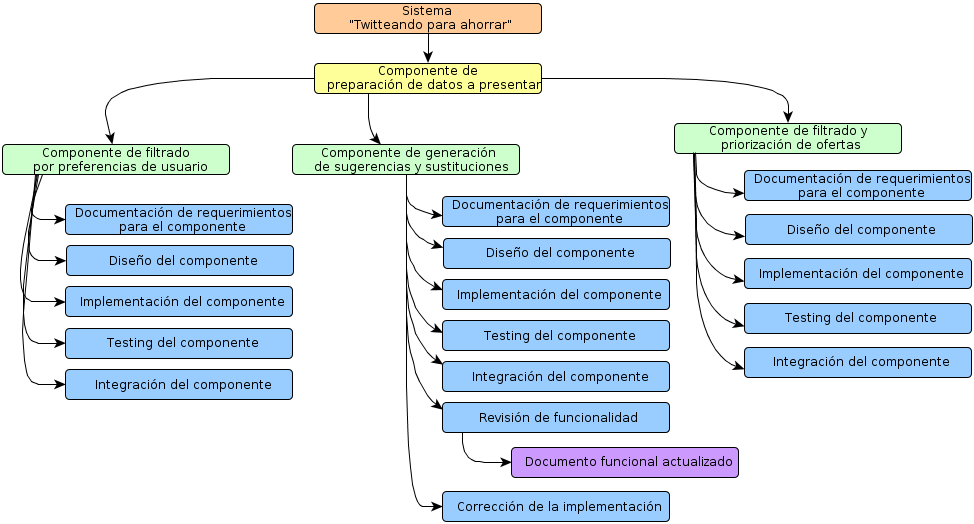
\includegraphics[width=\textwidth]{graficos/wbs/com_prep_de_datos.png}
\caption{Componente de preparación de datos a presentar}
\end{figure}

\begin{figure}[H]
\centering
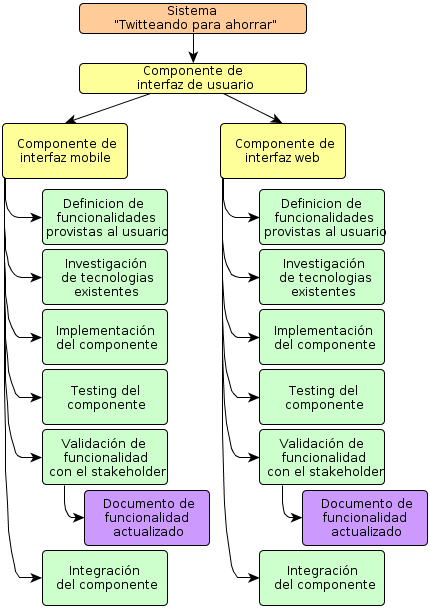
\includegraphics[scale=\escaladefault]{graficos/wbs/comp_interfaz.png}
\caption{Componente de interfaz de usuario}
\end{figure}

\begin{figure}[H]
\centering
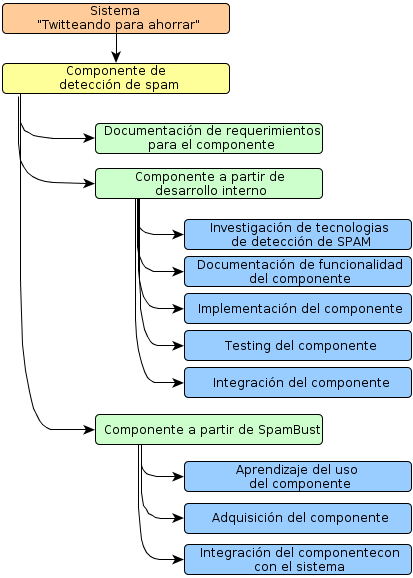
\includegraphics[scale=\escaladefault]{graficos/wbs/comp_de_spam.png}
\caption{Componente de detección de spam}
\end{figure}

\begin{figure}[H]
\centering
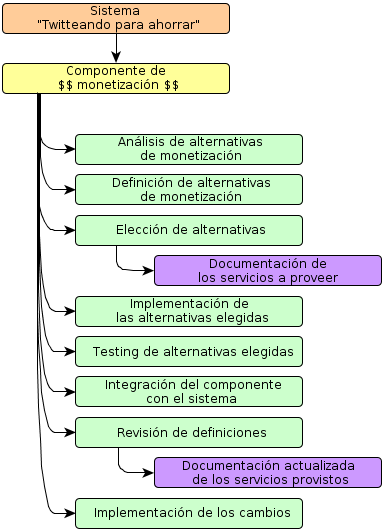
\includegraphics[scale=\escaladefault]{graficos/wbs/comp_monetizacion.png}
\caption{Componente de monetización}
\end{figure}

\begin{figure}[H]
\centering
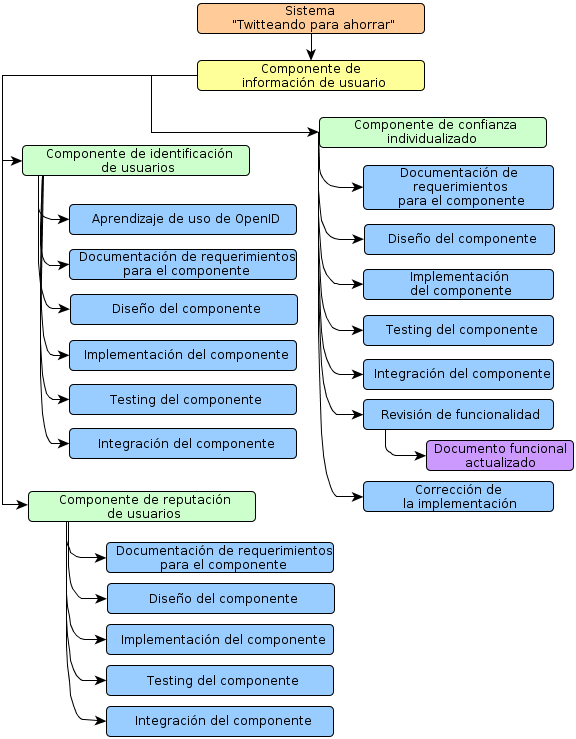
\includegraphics[scale=\escaladefault]{graficos/wbs/comp_de_info_de_usuario.png}
\caption{Componente de información de usuario}
\end{figure}


% hojas en landscape a partir de acá

\subsection{Plan detallado de la primera iteración}

Finalmente presentamos el plan detallado de la primera iteración. Aquí tenemos para cada uno de los componentes a desarrollar en la misma, el conjunto de tareas necesarias para lograrlos. Se encuentran definidas dependecias y estimaciones para cada una, por lo que puede verse exactamente la duración de la iteración. La misma tiene una duración de 6 semanas, lo cual deja tiempo \emph{colchón} para distintos inconvenientes que puedan originarse.

\begin{landscape}

\subsection{Plan de la primera iteración}

\begin{figure}[H]
\centering
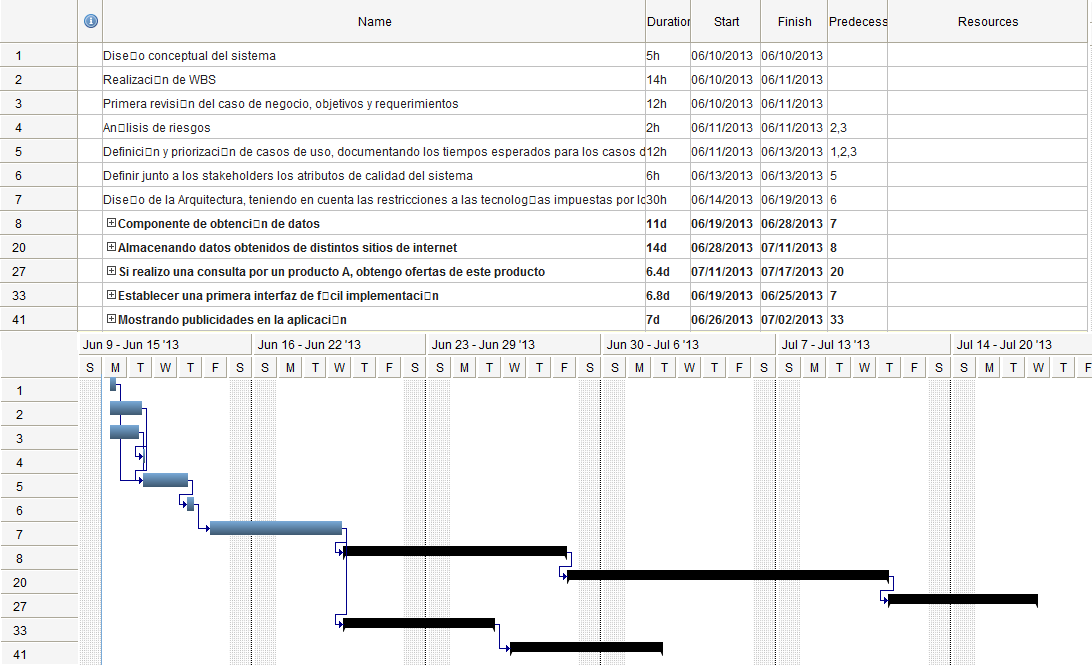
\includegraphics[scale=\escaladefault]{graficos/gantt/gantt.png}
\caption{}
\end{figure}

\begin{figure}[H]
\centering
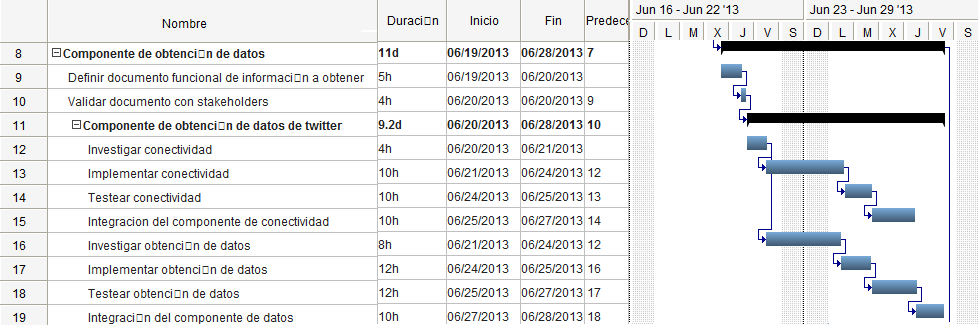
\includegraphics[scale=\escaladefault]{graficos/gantt/subgantt1.png}
\caption{}
\end{figure}

\begin{figure}[H]
\centering
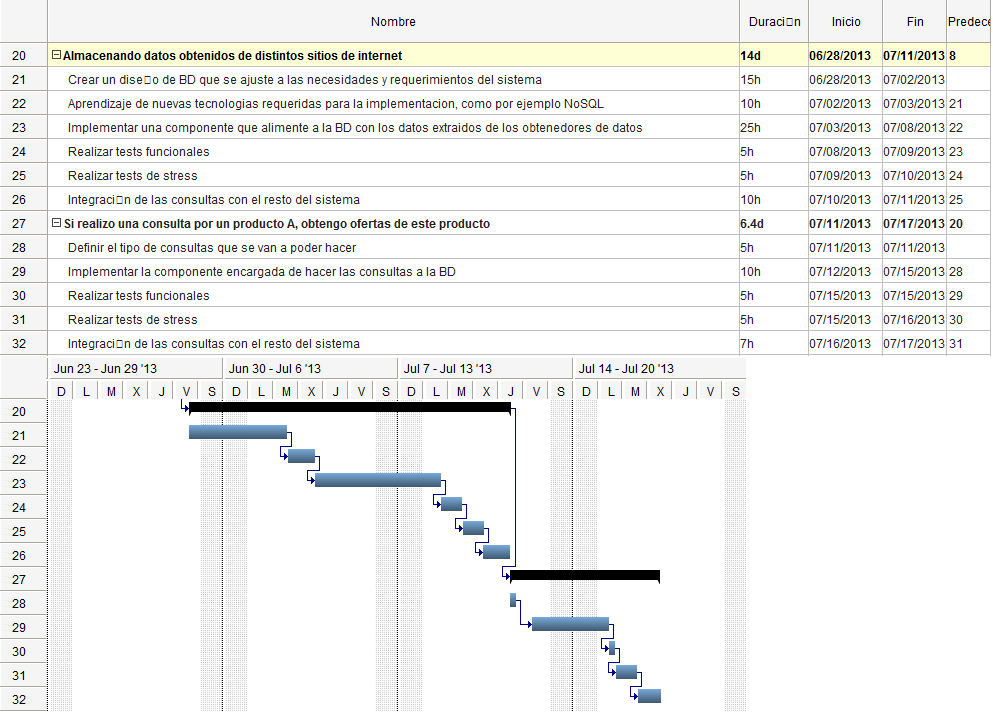
\includegraphics[scale=\escaladefault]{graficos/gantt/subgantt2.png}
\caption{}
\end{figure}

\begin{figure}[H]
\centering
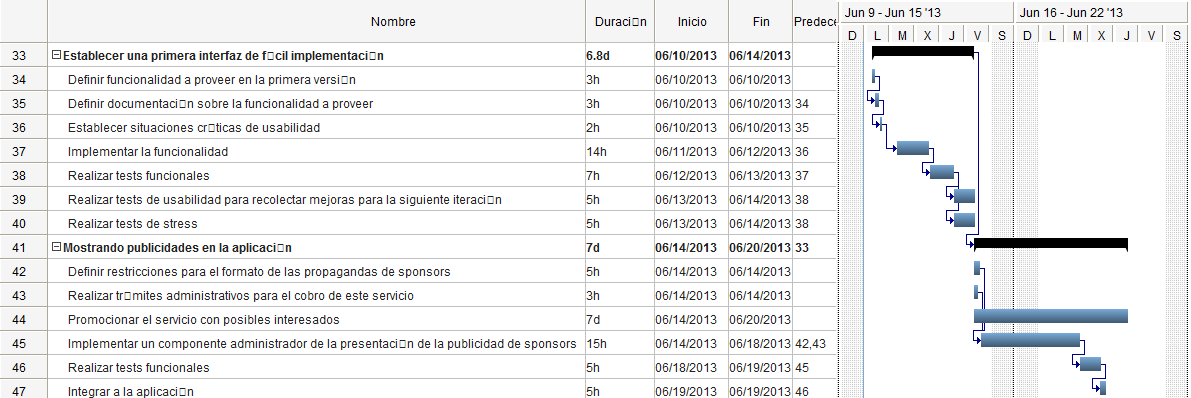
\includegraphics[scale=\escaladefault]{graficos/gantt/subgantt3.png}
\caption{}
\end{figure}

\end{landscape}


\end{document}
